%
% File coling2020.tex
%
% Contact: feiliu@cs.ucf.edu & liang.huang.sh@gmail.com
%% Based on the style files for COLING-2018, which were, in turn,
%% Based on the style files for COLING-2016, which were, in turn,
%% Based on the style files for COLING-2014, which were, in turn,
%% Based on the style files for ACL-2014, which were, in turn,
%% Based on the style files for ACL-2013, which were, in turn,
%% Based on the style files for ACL-2012, which were, in turn,
%% based on the style files for ACL-2011, which were, in turn, 
%% based on the style files for ACL-2010, which were, in turn, 
%% based on the style files for ACL-IJCNLP-2009, which were, in turn,
%% based on the style files for EACL-2009 and IJCNLP-2008...

%% Based on the style files for EACL 2006 by 
%%e.agirre@ehu.es or Sergi.Balari@uab.es
%% and that of ACL 08 by Joakim Nivre and Noah Smith

\documentclass[11pt]{article}
\usepackage{coling2020}
\usepackage{times}
\usepackage{url}
\usepackage{latexsym}
\renewcommand{\UrlFont}{\ttfamily\small}
\usepackage{graphicx}
\usepackage{tikz}
\usepackage{pgfplots}
\usepackage{subcaption}
\usepackage{url}
\usepackage{booktabs}
\usepackage{microtype}

% New command added by Hoang
\newcommand\BibTeX{B\textsc{ib}\TeX}
\newcommand{\argmax}[1]{\underset{#1}{\operatorname{arg}\,\operatorname{max}}\;}
\newcommand\footnoteref[1]{\protected@xdef\@thefnmark{\ref{#1}}\@footnotemark}
\newcommand{\todo}[1]{\textcolor{red}{TODO: #1}}
\newcommand{\comment}[1]{\textcolor{blue}{In Progress: #1}}



%\setlength\titlebox{5cm}
%\colingfinalcopy % Uncomment this line for the final submission

% You can expand the titlebox if you need extra space
% to show all the authors. Please do not make the titlebox
% smaller than 5cm (the original size); we will check this
% in the camera-ready version and ask you to change it back.


\title{AuSMeT: The Autocompletion for Simplifying Medical Text}

\author{First Author \\
  Affiliation / Address line 1 \\
  Affiliation / Address line 2 \\
  Affiliation / Address line 3 \\
  {\tt email@domain} \\\And
  Second Author \\
  Affiliation / Address line 1 \\
  Affiliation / Address line 2 \\
  Affiliation / Address line 3 \\
  {\tt email@domain} \\}

\date{}

\begin{document}
\maketitle
\begin{abstract}
  The goal of text simplification is to transform difficult text into a version that is easier to understand and more broadly accessible.  In some domains, such as healthcare and medical, fully automated approaches cannot be used since the information must be accurately preserved.  In this paper, we introduce the autocompletion task for text simplification, which aims to assist human simplification by suggesting the next word to type when manually simplifying a text.  We compare two pre-trained neural language models (BERT and GPT-2) and show how the additional context of the sentence to be simplified can be incorporated to achieve significantly better results (20.5\% and 28.8\% absolute improvement, respectively).  The best model, GPT-2 with context, achieves a word prediction rate of 52\% on Wikipedia data.

\end{abstract}

\section{Introduction}

Text simplification (TS) is the process of modifying the words and structure of a text while preserving the content to make the information in the text more broadly accessible \cite{shardlow2014survey}.  Most research in text simplification has focused on fully automated \cite{zhu10,coster2011learning,xu2016optimizing, zhang2017sentence,nishihara2019controllable}.  In some domains, e.g., medicine or healthcare, using fully-automated text simplifications is not appropriate since it is critical that the information gets preserved correctly during the simplification process. Instead of fully-automated approaches, support tools such as editors are better suited to generate simplifications more efficiently and with higher quality \cite{kloehn2018jmir}.

Autocompletion tools suggest one or more words as the user types that could follow what has been typed so far.  Autocompletion has been used in a range of applications including web queries \cite{cai2016survey}, database queries \cite{khoussainova2010snipsuggest}, texting \cite{dunlop2000predictive}, and e-mail composition \cite{dai2019gmail}. In this paper, we explore autocompletion for text simplification.  In contrast to most autocomplete applications, for text simplification, in addition to the text that is being typed, we also have the additional context of the content being simplified.  Our work is most similar to interactive machine translation tools where a user translating a foreign sentence is given guidance as they type \cite{green-etal-2014-human}.

In this paper, we examine the autocompletion task for sentence-level text simplification: given a difficult sentence that a user is trying to simplify and the simplification typed so far, the goal is to suggest the next word to follow what has been typed.  Figure \ref{fig:example} shows an example difficult sentence along with the simplification that the user has typed so far.  The task is to predict the next word to assist in finishing the simplification, in this case a verb like ``take'', which might be continued to a partial simplification of ``take place at the Chapel''.

\begin{figure}
    \centering
    \scalebox{0.9}{%
    \begin{tabular}{l l}
    \toprule
    Difficult & The Chapel is actively used as a place of\\
    sentence & worship and also for some concerts and\\
     & college events. \rule[-2ex]{0pt}{0pt} \\ 
    \hline
    Typed &  Concerts and college events $\rule{1cm}{0.15mm}$ \rule{0pt}{3ex} \\
    \bottomrule
    \end{tabular}}
    \caption{An example text simplification autocompletion task.  The user is simplifying the difficult sentence on top and has typed the words on the bottom so far.}
    \label{fig:example}
    \vspace{-0.15in}
\end{figure}

We make two main contributions.  First, we introduce the autocompletion task for sentence simplification and provide an initial analysis based on a number of recent models.  Second, we show how the additional context of the difficult sentence can be integrated into these models to improve the quality of the suggestions made.  Using the context of the difficult sentence significantly improves the prediction quality of the autocomplete methods.


\section{Text Simplification Autocomplete}

Given a difficult sentence that a user is trying to simplify, $d_1 d_2 ... d_m$, and the simplification typed so far, $s_1 s_2 ... s_i$, the autocompletion task is to suggest word $s_{i+1}$.   We examined two recent neural models that utilize the Transformer network \cite{vaswani2017attention}: BERT \cite{devlin2018bert} and GPT-2 \cite{radford2019language}.  The two models are state-of-the-art neural language representation models that have performed well in a range of applications.

To understand the benefit of the context of the difficult sentence, we compare models that do not use context, i.e., predict only based on $s_1 s_2 ... s_i$, and context-aware versions that incorporate the difficult sentence into the prediction.


%We view this problem as a language modeling problem and explored three different approaches, an $n$-gram language model and two pre-trained neural language models.   The neural language models allow for more context to be takent into account when making predictions and allow for us to incorporate the additional context of the difficult sentence.

\subsection{BERT}

%Neural language models use neural networks, often with many layers, to predict the likelihood of the next word given the context (and, in some cases, e.g., transformer models, actually predict the next word).  
%Unlike $n$-gram language models which are restricted to a fixed context, neural models use either recurrent neural networks \cite{mikolov2010recurrent}, Transformer networks, or other similar network configurations that build up an encoding of the context of the previous words and are therefore not limited to a fixed context window. 

BERT (Bidirectional Encoder Representations from Transformers) is a method for learning language representations using bidirectional training.  The main advantage of BERT is that it uses a masked approach to train the model where some of the words in the training data are replaced with a [MASK] token. The model then attempts to predict the original value of the masked words based on the context provided by the other, non-masked words in the sequence.  Unlike left-to-right or right-to-left sequential models, BERT can use context both before and after the word to be predicted.  BERT has been shown to produce state-of-the-art results in a wide range of generation and classification applications \cite{devlin2018bert}.

We use the original BERT pre-trained model, which was trained on the BooksCorpus \cite{zhu2015aligning} and English Wikipedia. To apply the model without context, we predict the masked word for the input ``$s_1 s_2 ... s_i \mbox{[MASK]} .$''. For the context-aware version, we add the context of the difficult sentence
``$d_1 d_2 ... d_m. s_1 s_2 ... s_i \mbox{[MASK]} .$''. This biases the prediction to words related to those found in the encoded context from difficult sentences.

BERT is a pre-trained model designed to be fine-tuned for particular applications. For the text simplification autocompletion task, we fine-tuned BERT on a corpus of sentence-aligned difficult concatenated with the corresponding simple sentences. We used Transformer Neural Networks to fine-tune the pre-trained BERT language model\footnote{\url{https://github.com/huggingface/transformers/tree/master/examples/}} on this data. Since, our task is to predict the next word in the simple sentence, we mask out each word in the simple sentence portion and then predict that word.

%\comment{This still needs to be clarified better.}

\subsection{GPT-2} 

Like BERT, GPT-2 is also based on the Transformer network, but uses left-to-right training and prediction. In each layer, GPT-2 has 12 independent attention mechanisms, called ``heads'', and the overall model contains 12 layers which can capture up to 144 different attention patterns.  We use the publicly released model\footnote{\url{https://github.com/openai/gpt-2}}, which has 1.5B model parameters and is trained on web text.  Since GPT-2 is a traditional left-to-right model, for the context unaware version we simply predict $s_{i+1}$ based on $s_1 s_2 ... s_i$.  Like BERT, to incorporate the context of the difficult sentence, we prepend it to the simplified text typed so far and then predict $s_{i+1}$.  We did not do any fine-tuning for GPT-2.

\section{Experiments} \label{sec:results}

We introduce a new task, text simplification autocomplete, which relies on a parallel corpus of difficult and simple sentences.  Given a difficult sentence and the the first $i$ words of the simple sentence, the goal is to predict the $i+1^{th}$ simple word.  We provide the first results on this task using BERT and GPT-2, with and without context, as well as an trigram language model baseline.

\subsection{Experimental setup}

To evaluate the quality of the different models, we used the Simple Wikipedia parallel corpus \cite{kauchak2013improving}, which contains 167K pairs of sentences, with one sentence from English Wikipedia and a corresponding sentence from Simple English Wikipedia.  We used 70\% of the sentence for training, 15\% for development, and 15\% for testing.

As an additional baseline that does not use context, we trained a trigram language model with Kneser-Ney smoothing using the SRILM toolkit \cite{stolcke2002srilm}.  The model was trainined on the simple sentences from the training portion of the dataset and predicts $s_{i+1}$ as the word with the highest probability given the previous two words, i.e., $argmax_{s_{i+1}}\mbox{ } p(s_{i+1}| s_i s_{i-1})$.

The BERT fine-tuning was done with a
batch-size of 8, 8 epochs, and a learning rate of $5e^{-5}$. Early stopping was used based on the second time a decrease in the accuracy was seen.

To evaluate the models, we calculated how well the models predicted the next word in a test sentence, given the previous words.  A simple test sentence of length $n$, $s_1 s_2 ... s_n$, would result in $n-1$ predictions, i.e., predict $s_2$ given $s_1$, predict $s_3$ given $s_1 s_2$, etc.  For example, Figure \ref{fig:testexample} shows a difficult sentence from English Wikipedia and the corresponding simplification from Simple English Wikipedia.  Given this test example, we generate six prediction tasks, one for each word in the simple sentence after the first word.  Figure \ref{fig:testing} shows these six test prediction tasks.  For the context-aware approaches, they also incorporated the difficult sentence. We measured the performance of a system using accuracy based on the number of predictions that exactly matched the next word in the corpus.  The test corpus contained 25K sentence pairs resulting in a total of 696K individual word predictions.

\begin{figure}
    \centering
    \scalebox{0.9}{%
    \begin{tabular}{l l}
    \toprule
    Difficult & The Saxons built Banbury on the west \\
    sentence & bank of the River Cherwell. \rule[-2ex]{0pt}{0pt} \\ 
    \hline
    Simple & Banbury is part of the Cherwell district. \rule{0pt}{3ex}\\
    sentence &  \\
    \bottomrule
    \end{tabular}}
    \caption{An example sentence pair from the English Wikipedia corpus.}
    \label{fig:testexample}
\end{figure}

\begin{figure}
\centering
\scalebox{0.9}{%
\begin{tabular}{ll}
\toprule \textbf{Typed so far} & \textbf{Predict} \\
\midrule
Banbury & is \\
Banbury is & part \\
Banbury is part & of \\
Banbury is part of & the \\
Banbury is part of the & Cherwell \\
Banbury is part of the Cherwell & district \\
\bottomrule
\end{tabular}}
\caption{The resulting prediction tasks that are generated from the example in Figure \ref{fig:testexample}.}
\label{fig:testing}
\vspace{-2mm}
\end{figure}

\begin{table}[t]
\centering
\scalebox{0.87}{%
\begin{tabular}{c c c }
\toprule
\textbf {Model} &\textbf{No Context} & \textbf {Context-Aware}\\ 
\midrule
trigram & 13\% & -- \\
\midrule
BERT & 21.5\% & 42\% \\
\midrule
%3 & RoBERTa & 22\% & 43\% \\
%\midrule
GPT-2 & 23.2\% & 52\% \\
\bottomrule
\end{tabular}}
\caption{Accuracy for the different models on the Wikipedia test corpus of 25K sentence pairs.  Context-aware approaches included the context of the difficult sentence when predicting.} 
\label{tab:results}
\vspace{-2mm}
\end{table}

\subsection{Prediction performance}
Table \ref{tab:results} shows the results for the five different variants (trigram model, BERT and GPT-2 with and without context).  Both neural models significantly outperform the trigram language model; they have been trained on larger corpora and have access to more context allowing for better predictions.  Without context, GPT-2 performs slightly better than BERT, with an absolute improvement of 1.7\%.  To put these accuracy numbers in perspective, in an actual autocomplete task, without context, both BERT and GPT-2 would get about every 4th or 5th word/suggestion correct.

With context, the results improve drastically and the accuracy rates double for both models.  The GPT-2 model benefits the most from the additional information with an absolute improvement of 28.8\% over the model without context, resulting in the best performing model with 52\% accuracy.  On the actual autocompletion task, this equates to predicting every other word correctly.  Note that this metric is pessimistic in that the predicted word must match exactly the word seen in the simple sentence and does not account for other possible words that could be correctly used in the context.

Table \ref{tab:context_information} shows the output of the GPT-2 model with and without context for simplifying the difficult sentence:

\vspace{-0.1in}
\begin{itemize}
    \item[] \textit{Each pseudostem can produce a single bunch of bananas.}
\end{itemize}

\vspace{-0.1in}

\noindent The context-aware version is able to take advantage of the strong overlap between the difficult sentence and the simplified version that is being ``typed''.  The model without context makes reasonable predictions grammatically, but without the content priming the suggestions are poor overall.

\begin{table*}[t]
\centering
\scalebox{0.85}{%
\begin{tabular}{l l l l}
\toprule 
& \multicolumn{2}{c}{\textbf{GPT-2}} & \\
\textbf{Typed so far} & \textbf{No Context} & \textbf{Context-Aware} & \textbf{Actual}\\
\midrule
A & particle & \textbf{pseudostem} & \textbf{pseudostem} \\
A pseudostem & was & \textbf{is} & \textbf{is} \\
A pseudostem is & a & \textbf{able} &  \textbf{able} \\
A pseudostem is able & \textbf{to} & \textbf{to} & \textbf{to} \\
A pseudostem is able to & create & \textbf{produce} & \textbf{produce} \\
A pseudostem is able to produce & \textbf{a} & \textbf{a} & \textbf{a} \\
A pseudostem is able to produce a & new & \textbf{single} & \textbf{single} \\
A pseudostem is able to produce a single & photon &\textbf{bunch} & \textbf{bunch} \\
A pseudostem is able to produce a single bunch & \textbf{of} & \textbf{of} & \textbf{of} \\
A pseudostem is able to produce a single bunch of & particles & \textbf{bananas} &  \textbf{bananas} \\
\bottomrule
\end{tabular}}
\caption{\label{tab:context_information} Sample output for simplifying the difficult sentence ``\textit{Each pseudostem can produce a single bunch of bananas.}'' using GPT-2 with and without context.  ``Actual'' indicates the word that should be predicted.}
\vspace{-2mm}
\end{table*}

\subsection{Understanding model performance}

To better understand how the models are performing and how the predictions of the models differ, we broke down the performances of the neural models by part of speech (POS), difficult sentence length, and the number of words typed so far.

\vspace{-1mm}
\paragraph{POS} Table \ref{tab:POS-results} shows the accuracies broken down by part of speech, where the POS was automatically determined using Stanford CoreNLP  \cite{manning2014corenlp}.  All of the models perform best on non-content bearing words (i.e., ``Other'').  Of the content-bearing words, the models did the best on verbs and the worst on adverbs.  Overall, GPT-2 with context was the best model at predicting content words with all of the accuracies above 40\% except for adverbs, which was 37\%.

\begin{table}[t]
\centering
\scalebox{0.76}{%
\begin{tabular}{l c c c c c}
\toprule
 & & \multicolumn{2}{c}{\textbf{No Context(\%)}} & \multicolumn{2}{c}{\textbf{Context-Aware(\%)}} \\
 & N & BERT & GPT-2 & BERT & GPT-2\\
 \midrule
All words & 696,683 & 22 & 23 & 42 & 52\\
\midrule
Nouns & 301,363 & 13 & 15 & 33 & 43\\
Verbs & 80,180 & 16 & 17 & 39 & 47 \\
Adverbs & 23,600 & 10 & 9 & 25 & 37\\
Adjectives & 41,780 & 10 & 11 & 30 & 46\\
Other & 249,760 & 32 & 31 & 71 & 60 \\
 \bottomrule
\end{tabular}}
\caption{\label{tab:POS-results} Accuracy of the BERT and GPT-2 with and without context by part-of-speech on the test data.}
\vspace{-2mm}
\end{table}

%First and most important, the results demonstrate that our approach can be used to simplify text given difficult sentence. The best performance is from GPT-2 (see table \ref{tab:results} line 4 column 3). Our proposed models: using pretrained language models BERT, and GPT-2 outperform baseline performance by 8-10\% given the same amount of information classified as non-context-aware. This also suggests that our approach can be used to provide real-time suggestion for text simplification as opposed to other approaches, which simply replace difficult vocabularies with simpler ones. 

%Our analysis with the parts of speech on the prediction results of our models shows that we achieve highest performance improvement on predicting adjectives of a sentence (318\%) using GPT-2 with context (Table \ref{tab:POS-results}).

%\textbf{Impact of context information:} With context information from normal sentence combined with each input to our model, the performance is improved significantly by 19-21\% (see column Context-Aware in table \ref{tab:results}). This suggests that the contextual information from normal sentence can be used to predict the next word in the simple sentence. Table \ref{tab:context_information} shows an example of GPT-2 predictions with and without context. Combining with normal sentence, it allows our model to learn specific context in need of simplification, resulting better prediction as compared to non-context-aware. Since n-gram models are statistics-based and only allow fix amount of previous words, these models are not applicable for context-aware information. However, the significant differences between non-context-aware and context-aware performances of BERT, and GPT-2 suggests the significant impact of these information on model performance.

\vspace{-1mm}
\paragraph{Difficult sentence length} Figure \ref{fig:length_based} shows the performance of the context-aware models based on the length of the difficult sentence.  BERT is fairly consistent regardless of the length of the difficult sentence.  Only for very long sentences does the performance drop.  GPT-2 performs poorly on very short sentences, but well for other lengths.  We hypothesize that the training data for GPT-2 (web text) may require more context for the more technical Wikipedia task. 

\begin{figure}[t]
\center{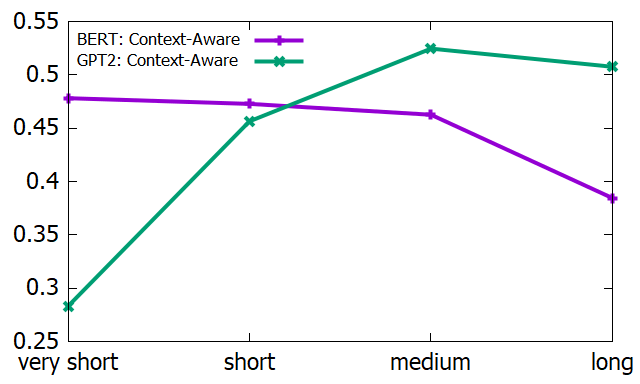
\includegraphics[width=\linewidth]
{./images/new_len_fig.png}}
\caption{\footnotesize \label{fig:length_based} Accuracy for the two context-aware models based on the length of the difficult sentence: very short ($\le 5$ tokens), short ($6-15$), medium ($16-19$), and long ($\ge20$).}
\vspace{-2mm}
\end{figure}

\begin{figure}[t]
\center{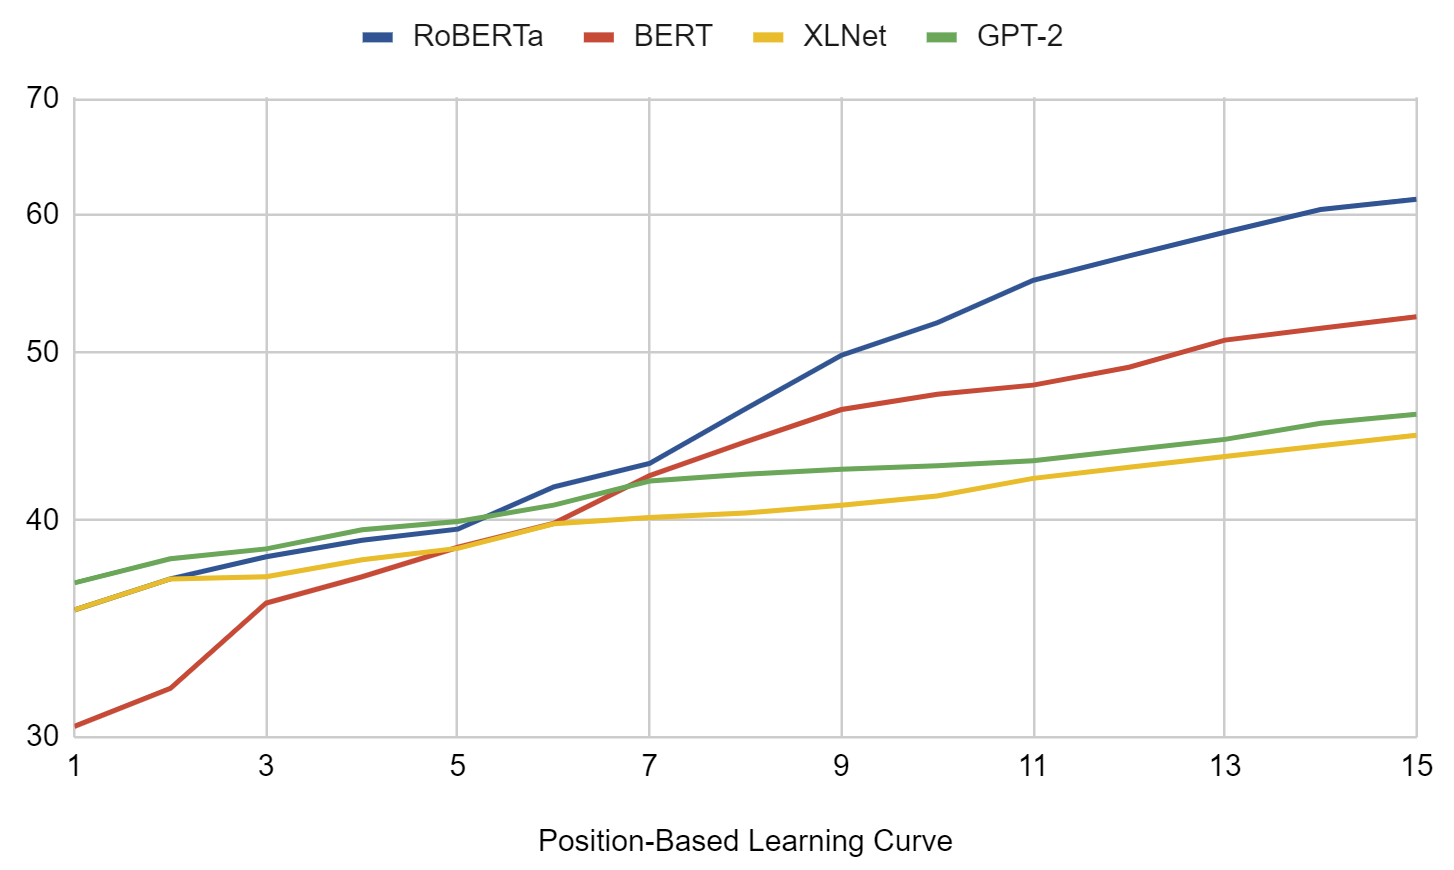
\includegraphics[width=\linewidth]
{./images/new_pos_fig.png}}
\caption{Accuracy for the two context-aware models based on the number of words typed so far ($i$).}
\label{fig:position_based}
\vspace{-2mm}
\end{figure}

\vspace{-1mm}
\paragraph{Number of words typed}
Figure \ref{fig:position_based} shows the performance of the two context-aware models based on how many words of the simplification the model has access to, i.e., $i$.  Early on when the sentence is first being developed, both models struggle.  As more and more words are typed and more context is provided, the accuracy of both models increase, however, GPT-2 improves more rapidly as additional context is provided. Like the difficult sentence length analysis, GPT-2 performs better with more context information.

%concludes our hypothesis that the further we go along the sentence, the better the prediction of next word from our models. From position 1 to position 10, the performance of BERT increases by 5.9\% (35.53\% to 41.43\%) while GPT-2 gains roughly 15\% (39.43\% to 54.56\%). This observation again confirms our hypothesis that GPT can better capture longer context information; however, in this experiment, in the simplified sentence itself. 

%Another important observation from figure \ref{fig:position_based} is that the improvements decrease as we go further along the simplified sentences. Within the first couple words (see Figure \ref{fig:position_based} position 0 to 4), the improvement is larger as composed to the later positions (position 8 to 10). This observation also suggests that the model can quickly learn the context information and make better prediction. Once again, this concludes that our approach can be used to provide real-time suggestion for TS.   

\section{Conclusions}

In this paper we have introduced a new task, text simplification autocompletion.  Unlike most autocomplete tasks, for text simplification, models can be guided by the sentence that the user is simplifying.  We compared two recent neural models, BERT and GPT-2, and showed how the difficult sentence could be incorporated into the prediction process.  Using context resulted in significant increases in performance with the best model, GPT-2 with context, achieving a prediction accuracy of 52\%, getting every other word right.  We hope that this new task will allow for other interesting model adaptations to be explored.


%%%%%%%%%%%%%%%End of content%%%%%%%%%%%%%%%
% Added it back on for Sponsor Acknowledgements
%\section*{Acknowledgements}

%The acknowledgements should go immediately before the references.  Do not number the acknowledgements section. Do not include this section when submitting your paper for review.

% include your own bib file like this:
\bibliographystyle{coling}
\bibliography{coling2020}

%\begin{thebibliography}{}

%\bibitem[\protect\citename{Aho and Ullman}1972]{Aho:72}
%Alfred~V. Aho and Jeffrey~D. Ullman.
%\newblock 1972.
%\newblock {\em The Theory of Parsing, Translation and Compiling}, volume~1.
%\newblock Prentice-{Hall}, Englewood Cliffs, NJ.

%\bibitem[\protect\citename{{American Psychological Association}}1983]{APA:83}
%{American Psychological Association}.
%\newblock 1983.
%\newblock {\em Publications Manual}.
%\newblock American Psychological Association, Washington, DC.

%\bibitem[\protect\citename{{Association for Computing Machinery}}1983]{ACM:83}
%{Association for Computing Machinery}.
%\newblock 1983.
%\newblock {\em Computing Reviews}, 24(11):503--512.

%\bibitem[\protect\citename{Chandra \bgroup et al.\egroup }1981]{Chandra:81}
%Ashok~K. Chandra, Dexter~C. Kozen, and Larry~J. Stockmeyer.
%\newblock 1981.
%\newblock Alternation.
%\newblock {\em Journal of the Association for Computing Machinery},
%  28(1):114--133.

%\bibitem[\protect\citename{Gusfield}1997]{Gusfield:97}
%Dan Gusfield.
%\newblock 1997.
%\newblock {\em Algorithms on Strings, Trees and Sequences}.
%\newblock Cambridge University Press, Cambridge, UK.

%\bibitem[\protect\citename{Rasooli and Tetreault}2015]{rasooli-tetrault-2015}
%Mohammad~Sadegh Rasooli and Joel~R. Tetreault. 2015.
%\newblock {Yara parser: {A} fast and accurate dependency parser}.
%\newblock \emph{Computing Research Repository}, arXiv:1503.06733.
%\newblock Version 2.

%\bibitem[\protect\citename{Borschinger and Johnson}2011]{borsch2011}
%Benjamin Borschinger and Mark Johnson. 2011.
%\newblock A particle filter algorithm for {B}ayesian wordsegmentation.
%\newblock In \emph{Proceedings of the Australasian Language Technology Association %Workshop 2011}, pages 10--18, Canberra, Australia.

%\end{thebibliography}

\end{document}
